%\newcommand{\Exp}{\mathbb{E}}

% reset section counter
\setcounter{section}{0}

%\metadata{lecture ID}{Your names}{date}
\metadata{6}{Louie Kam and Shaan Patel}{May 7th, 2021}

\sec{Review and overview}
In the previous lecture, we began our discussion on neural nets and claimed that neural nets are equivalent to nonparametric penalized regression for one dimensional inputs; specifically, we showed that there exists a complexity measure $\bar{R}(f)$ for nonparametric penalized regression such that the nonparametrized penalized regression minimization problem is the same as the parametrized neural network one, i.e. $\min_{f}L(f) + \lambda \bar{R}(f) = \min_{\theta} L(h_\theta) + \lambda C(\theta)$.

In this lecture, we will discuss the next step of the proof by deriving an explicit formula for $\bar{R}(f)$. Following that, we will take a look at algorithms that will solve this minimization problem and discuss the intuition behind them. In particular, we will discuss gradient descent methods and feature training.
\sec{Finishing up proof}

\subsec{Recap}
Recall from the last lecture, we introduced the following quantities for an infinitely-wide two-layer neural net,
\begin{align*}
a & = (a_1, a_2, a_3, \cdots) \in \bbR^\infty, \\
b & = (b_1, b_2, b_3, \cdots) \in \bbR^\infty, \\
w & = (w_1, w_2, w_3, \cdots) \in \bbR^\infty, \\
h_\theta(x) & = \sum_{i=1}^\infty a_i [w_ix+b_i]_+, \\
C(\theta) &= \frac{1}{2} \bigg(\sum_{i=1}^\infty a_i^2 + \sum_{i=1}^\infty w_i^2\bigg).
\end{align*}
Denote $\theta$ as the set of vectors $\{(a_i, b_i, w_i)\}_{i=1}^\infty$. In the previous lecture, we posted the following theorem.

\begin{theorem}\label{thm:eq}
Let $\bar{R}(f)$ be a complexity measure such that
\al{\label{eqn:measure}
\bar{R}(f) \overset{\Delta}{=} \max\bigg\{\int_{-\infty}^\infty |f''(x)|, |f'(-\infty)+f'(+\infty)|\bigg\}.
}
 Let $f^*$ to be the nonparametric penalized regression that minimizes
\[
\min_f L(f)+\lambda\bar{R}(f).
\]
 Let $h_{\theta^*}$ be the parametric neural net that minimizes
\[
\min_\theta L(h_\theta)+\lambda C(\theta).
\]
Then $f^* = h_{\theta^*}$ and 
\al{\label{eqn:min_eq}
\min_f L(f)+\lambda\bar{R}(f) = \min_\theta L(h_\theta)+\lambda C(\theta).
}
\end{theorem}

 We previously showed that there exists
\al{\label{eqn:rf}
\bar{R}(f) \overset{\Delta}{=} \min C(\theta) \quad \text{ s.t. } \quad f(x) = h_\theta(x),
}
and Eq.~\eqref{eqn:min_eq} holds for this definition of $\bar{R}(f)$. It remains to show the definition of complexity measure in Eq.~\eqref{eqn:min_eq} holds for \eqref{eqn:rf}. Let us take a detour and prove a related lemma.

\subsec{Preparation}

\begin{lemma}\label{lemma:a=w}
The minimizer $\theta^*$ of Eq.~\eqref{eqn:rf} satisfies $|a_i| = |w_i|$, for all $i = 1, 2, \cdots$. 
\end{lemma}

Recall that the $w_i$'s are the weights of the first layer and the $a_i$'s are the weights of the second layer. Therefore, this lemma implies that the weights are balanced between the two levels in order to minimize the complexity.

\begin{proof}
	We can write $a_i[w_ix + b_i]_+ = \frac{a_i}{\gamma}[\gamma w_ix + \gamma b_i]_+$ if $\gamma > 0$. This is allowed because $[\gamma t]_+ = \gamma[t]_+$.
	Now suppose that $(a_i,w_i,b_i)$ is optimal for each $i$. Then the complexity should not decrease after scaling by $\gamma$ as we have already found the minimum.
	\begin{equation}
		\frac{1}{2}(a_i^2 + w_i^2) \leq \frac{1}{2}(\frac{a_i^2}{\gamma^2} + \gamma^2 w_i^2).
	\end{equation}
	Now we minimize with respect to $\gamma$.
	\begin{equation}
		\min_{\gamma} \frac{1}{2}(\frac{a_i^2}{\gamma^2} + \gamma^2 w_i^2) = \frac{1}{2}(a_i^2 + w_i^2).
	\end{equation}
	Let $g(\gamma) = \frac{1}{2}(\frac{a_i^2}{\gamma^2} + \gamma^2 w_i^2)$. Therefore $\min g(\gamma) = g(1)$.
	\begin{align*}
		& g'(1) = 0 = \frac{-a_i^2}{\gamma^3} + \gamma w_i^2 = -a_i^2 + w_i^2 \\
		& \Rightarrow a_i^2 = w_i^2 \\
		& \Rightarrow |a_i| = |w_i|.
	\end{align*}
\end{proof} 
 We now proceed to finish our proof of Theorem \ref{thm:eq}. We can redefine our neural net $h_\theta(x)$: 
\[
\begin{split}
h_\theta(x) &= \sum_{i=1}^\infty a_i [w_ix+b_i]_+ = \sum_{i=1}^\infty a_i |a_i| \bigg[\frac{w_i}{|a_i|} x + \frac{b_i}{|a_i|}\bigg]_+ = \sum_{i=1}^\infty \alpha_i [\widetilde w_i x + \beta_i]_+,
\end{split}
\]
where $\alpha_i = a_i |a_i|$, $\widetilde w_i = \frac{w_i}{|a_i|}$, and $\beta_i = \frac{b_i}{|a_i|}$. Since $\theta$ satisfies Eq.~\eqref{eqn:rf}, by using the results of Lemma \ref{lemma:a=w}, we know that $\alpha_i \in \{-a_i^2, a_i^2\}$ and $\widetilde w_i \in \{-1, 1\}$. Furthermore, we can redefine $C(\theta)$:
\[
\begin{split}
C(\theta) &= \frac{1}{2} \bigg(\sum_{i=1}^\infty a_i^2 + \sum_{i=1}^\infty w_i^2\bigg) = \frac{1}{2} \bigg(\sum_{i=1}^\infty a_i^2 + \sum_{i=1}^\infty a_i^2\bigg) = \sum_{i=1}^\infty a_i^2 = \sum_{i=1}^\infty |\alpha_i|.
\end{split}
\]
Define a new neural net by the set of parameters $\widetilde \theta = \{(\alpha_i, \beta_i, \widetilde w_i)\}_{i=1}^\infty$. Then the objective function in Eq.~\eqref{eqn:rf} becomes
\al{\label{eqn:rf_1}
R(f) \overset{\Delta}{=} \min \norm{\alpha}_1 \quad \text{ s.t. } \quad f(x) = h_{\widetilde \theta}(x).
}

\subsec{Discretization to rewrite $h_{\widetilde\theta}(x)$}
The neural net $h_{\widetilde \theta}(x)$ can be grouped by whether $\widetilde w_i = 1$ and $\widetilde w_i = -1$:
\[
h_{\widetilde\theta}(x) = \sum_{i: \widetilde w_i = 1} \alpha_i [x+\beta_i]_+ + \sum_{i: \widetilde w_i = -1} \alpha_i [-x+\beta_i]_+
\]
Let $Z=\{z_1, \cdots, z_N\}$ be a discretization of $\bbR$. Then $[x+\beta_i]_+$ can be approximated by $[x+z_j]_+$, where the bin around $z_j$ is the ``bucket'' that $\beta_i$ falls into. Since $[x+z_j]_+$ is constant over all $i$ where $\beta_i$ falls into $z_j$, we can isolate $\alpha$ such that
\[
\sum_{i: \beta_i \in z_j} \alpha_i [x+\beta_i]_+ \approx [x+z_j]_+ \sum_{i: \beta_i \in z_j} \alpha_i.
\]
Similar logic holds for $[-x+z_j]_+$. See Fig.~\ref{fig:disc} for an example of discretization. 
\begin{figure}[h]
\centering
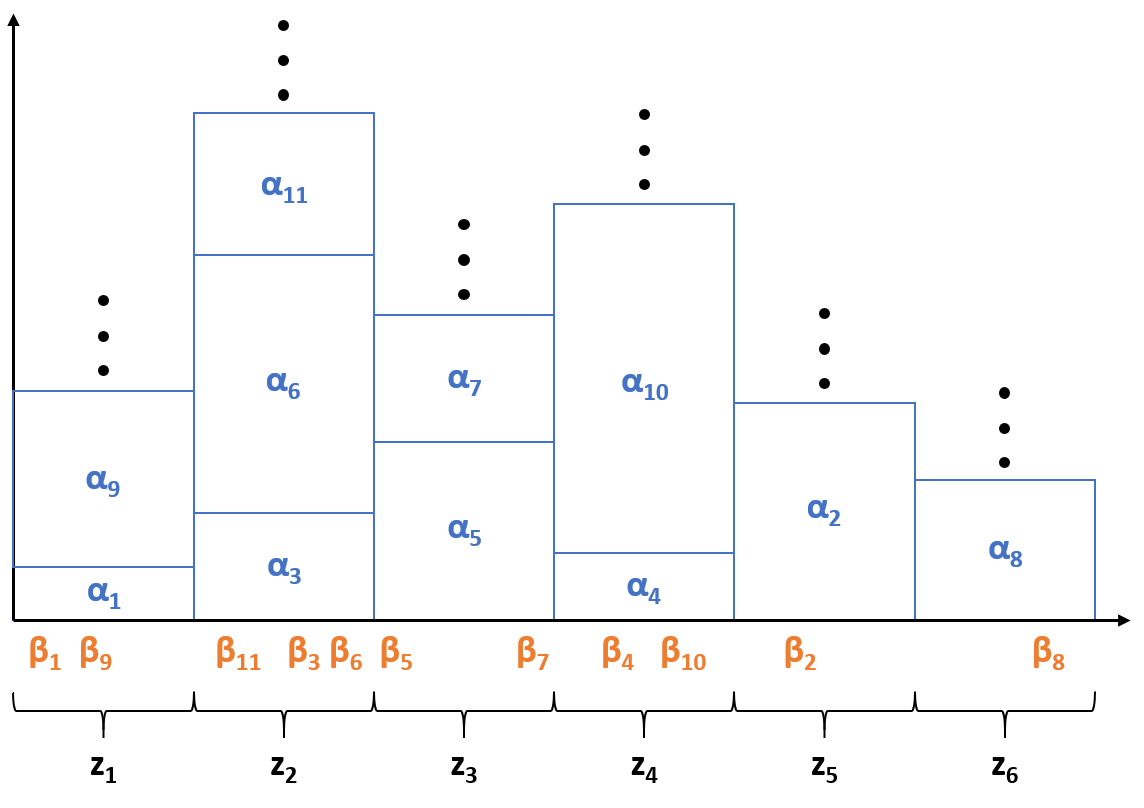
\includegraphics[width=0.8\textwidth]{figure/Lecture06/discretization.png}
\caption{Example of discretization across $\bbR$} \label{fig:disc}
\end{figure}

Define $u^+(z)$ and $u^-(z)$ as
\[u^+(z)=\bigg(\sum_{i:\widetilde w_i = 1, \beta_i = z} \alpha_i\bigg), u^-(z)=\bigg(\sum_{i:\widetilde w_i = -1, \beta_i = z} \alpha_i\bigg).
\]
Then
\[
\sum_{i: \widetilde w = 1} \alpha_i [x+\beta_i]_+ = \sum_{z \in Z} [x+z]_+ \bigg(\sum_{i:\widetilde w_i = 1, \beta_i = z} \alpha_i\bigg) = \sum_{z \in Z} [x+z]_+ u^+(z),
\]
and thus we have 
\[
h_{\widetilde\theta}(x) = \sum_{z \in Z} [x+z]_+ u^+(z) + \sum_{z \in Z} [-x+z]_+ u^-(z).
\]
Taking the limit $N\to\infty$ makes the discretization fine-grained and results in the integral,
\[
h_{\widetilde\theta}(x) = \int_{-\infty}^\infty [x+z]_+ u^+(z) dz + \int_{-\infty}^\infty [-x+z]_+ u^-(z) dz.
\]
We can view $h_{\widetilde\theta}(x)$ as a linear combination of features $[x+z]_+$ and $[-x+z]_+$ for $z \in \bbR$.

\subsec{Reformulation of the objective}
 We know that
\[
\sum_{i=1}^\infty |\alpha_i| \ge \int_{-\infty}^{\infty} |u^+(z)| dz + \int_{-\infty}^{\infty} |u^-(z)| dz.
\]
by the triangle equality; for every bucket $z$, $\sum_{i: \beta_i \in z} |\alpha_i| \ge |u^+(z)| = |\sum_{i: \beta_i \in z} \alpha_i|$ and a similar expression holds for $u^-(z)$. Equality occurs at the minimum, as the optimal $\theta$ minimizes complexity regardless of how we rewrite the expression. Thus, we can update our objective in Eq.~\eqref{eqn:rf_1}:
\al{\label{eqn:rf_2}
\min \int_{-\infty}^{\infty} |u^+(z)| dz + \int_{-\infty}^{\infty} |u^-(z)| dz \quad \text{ s.t. } \quad f(x)=h_{\widetilde\theta}(x).
}
We can write the first derivative of $[x+z]_+$ to be
\[
\frac{d}{dx} [x+z]_+ = I(x+z \ge 0),
\]
and the second derivative of $[x+z]_+$ to be
\[
\frac{d}{dx} I(x+z \ge 0) = \delta_{-x}(z) = 
\begin{cases}
\infty & \text{if } z=-x \\
0 & \text{otherwise}
\end{cases}.
\]
Likewise, the first derivative of $[-x+z]_+$ is
\[
\frac{d}{dx} [-x+z]_+ = -I(-x+z \ge 0),
\]
and the second derivative of $[-x+z]_+$ is
\[
\frac{d}{dx} [-I(-x+z \ge 0)] = \delta_{x}(z) = 
\begin{cases}
\infty & \text{if } x=z \\
0 & \text{otherwise}
\end{cases}.
\]
The derivative of $f(x)$ is
\[
f'(x) = h_{\widetilde\theta}'(x) = \int_{-\infty}^{\infty} I(x+z \ge 0) u^+(z) dz + \int_{-\infty}^{\infty} -I(-x+z \ge 0) u^-(z) dz,
\]
and the derivative of $f'(x)$ is
\[
f''(x) = \int_{-\infty}^\infty \delta_{-x}(z) u^+(z) dz + \int_{-\infty}^\infty \delta_{x}(z) u^-(z) dz = u^+(-x) + u^-(x).
\]
Note that the last equality holds because $\delta_{-x}(z)$ and $\delta_{x}(z)$ can be treated as ``degenerate'' probability distributions (with total probability 1 occurring only at $-x$ and $x$, respectively). Our choice of $x$ was arbitrary, so this holds for all $x$. Thus, the objective from Eq.~\eqref{eqn:rf_2} becomes
\al{\label{eqn:rf_3}
\min \int_{-\infty}^{\infty} |u^+(z)| dz + \int_{-\infty}^{\infty} |u^-(z)| dz \quad \text{ s.t. } \quad \forall x, f''(x) = u^+(-x) + u^-(x).
}

\subsec{Simplification of the constraints}
We can further remove redundancies by parameterizing $u^+(-x)$ and $u^-(x)$ in terms of a function $q$ and using the constraint $f''(x) = u^+(-x) + u^-(x)$:
\[
\begin{split}
u^+(-x) &= \frac{1}{2}(f''(x) - q(x)), \\
u^-(x) &= \frac{1}{2}(f''(x) + q(x)).
\end{split}
\]
Then the objective function in Eq.~\eqref{eqn:rf_3} can be written as
\[
\begin{split}
\int_{-\infty}^{\infty} |u^+(z)| dz + \int_{-\infty}^{\infty} |u^-(z)| dz &= \int_{-\infty}^{\infty} |u^+(-z)| dz + \int_{-\infty}^{\infty} |u^-(z)| dz \\
&= \int_{-\infty}^{\infty} \Big|\frac{1}{2}(f''(z) - q(z))\Big| dz + \int_{-\infty}^{\infty} \Big|\frac{1}{2}(f''(z) + q(z))\Big| dz \\
&= \frac{1}{2} \int_{-\infty}^\infty \Big(|f''(z)-q(z)| + |f''(z)+q(z)|\Big) dz.
\end{split}
\]
Since $|f''(z)-q(z)| + |f''(z)+q(z)|$ is $2|f''(z)|$ if $|f''(z)| \ge q(z)$ and $2|q(z)|$ if $|f''(z)| < q(z)$, we have a simple expression for the objective function:
\[
\int_{-\infty}^{\infty} |u^+(z)| dz + \int_{-\infty}^{\infty} |u^-(z)| dz = \int_{-\infty}^\infty \max\{|f''(z)|, |q(z)|\} dz.
\]
We can find a constraint on $q$ using
\[
f'(x) = \int_{-\infty}^{\infty} I(x+z \ge 0) u^+(z) dz + \int_{-\infty}^{\infty} -I(-x+z \ge 0) u^-(z) dz,
\]
specifically the values of $f'(-\infty)$ and $f'(\infty)$:
\[
\begin{split}
f'(-\infty) &= \int_{-\infty}^{\infty} -u^-(z) dz = \int_{-\infty}^{\infty} -\frac{1}{2}(f''(z) + q(z)) dz, \\
f'(\infty) &= \int_{-\infty}^{\infty} u^+(z) dz = \int_{-\infty}^{\infty} u^+(-z) dz = \int_{-\infty}^{\infty} \frac{1}{2}(f''(z) - q(z)).
\end{split}
\]
Thus, the sum
\al{
f'(-\infty) + f'(\infty) = - \int_{-\infty}^\infty q(z) dz
}
gives a constraint for $q$, and we update the objective in Equation \ref{eqn:rf_3} in terms of $q$:
\al{\label{eqn:rf_4}
\min \int_{-\infty}^{\infty} \max\{|f''(z)|, |q(z)|\} dz \text{ s.t. } f'(-\infty) + f'(\infty) = - \int_{-\infty}^\infty q(z) dz.
}
Previous formulations of the objective were taken with respect to many (infinite) variables, but we have found an equivalent objective with respect to $q$ only. Consider the following discrete objective
\[
\min \sum_{i=1}^k \max\{a_i, |x_i|\} \quad \text{ s.t. } \quad \sum_{i=1}^k x_i = B.
\]
The minimum value of the objective function above is $\max\{\sum_{i=1}^k a_i, |B|\}$. Connecting this idea to our objective in Equation \ref{eqn:rf_4}, the minimum value of the objective function is 
\[
\max\bigg\{\int_{-\infty}^\infty |f''(x)|, |f'(-\infty) + f'(\infty)|\bigg\},
\]
which is $\bar{R}(f)$ for the initial objective in Eq.~\eqref{eqn:rf} so we are done.

\sec{Optimization}

\subsec{Basic Premise}

In a general sense, our neural network function is of the form
$$
h_\theta(x) = a^T \phi_w(x).
$$
where $\phi_w(x)$ has a lot of layers in it. We established the conventional viewpoint that the earlier layers of $\phi_w(x)$ are producing features and the last layer is producing some linear classification of all of them. The typical objective function for regression is then denoted by
\begin{align}
L(\theta) = \min \frac{1}{2n}\sum_{i=1}^n (y^{(i)} - h_\theta(x^{(i)}))^2 + \frac{\lambda}{2} \left\| \theta \right\|_2^2. \label{eqn:loss}
\end{align}
We want to find some algorithms that will help us solve this optimization problem.

\subsec{Gradient Descent}
Let us start from some initialization $\theta_0$. This initialization is often random but the exact initialization, or rather the scale, matters. After the initialization is created with an initial set of parameters we take the gradient and do a recursion.
$$
\theta_{t+1} = \theta_t - \eta \nabla L(\theta_t).
$$

Why does this work? In essence, we are finding the steepest descent at a point $\theta_t$ and moving in that direction. If we look at a Taylor expansion of $L(\theta)$ at the point $\theta_t$, we get
$$
L(\theta) = L(\theta_t) + \langle \nabla L(\theta_t), \theta - \theta_t \rangle + \text{higher order terms}.
$$
Notice that the second term is linear in $\theta$. If we ignore the higher order terms and minimize over a Euclidean ball around $\theta_t$ (the ball is required to maintain the accuracy of the Taylor expansion), we get
$$
\argmin L(\theta_t) +  \langle \nabla L(\theta_t), \theta - \theta_t \rangle, \qquad s.t. \qquad \| \theta - \theta_t \|_2 \leq \varepsilon
$$
$L(\theta_t)$ is a constant in this case, so this simplifies to
$$
\min \langle \nabla L(\theta_t), \theta - \theta_t \rangle, \qquad s.t. \| \theta - \theta_t \|_2 \leq \varepsilon
$$
This is equivalent to finding two vectors $v$ and $x$ with minimum correlation such that $x$ has norm less than $\varepsilon$. As a result, the optimal solution is  $x = -cv$, where $c$ is a scalar constant greater than 0. This assures that our two vectors have a minimum correlation as they are in opposite directions, and $c$ allows the vector to be within our previously established ball. Therefore the optimal solution for $\theta - \theta_t$ is 
$$
\theta - \theta_t = -c\cdot \nabla L(\theta_t)
$$
Therefore, we can see that the steepest direction is optimal, and thus the gradient descent method will reach a minimum.

\subsec{Stochastic gradient descent}
For many machine learning problems, computing the gradient is a computationally expensive task. Consider the gradient for the loss function in Eq.~\eqref{eqn:loss}:
\[
\nabla L(\theta_t) = \frac{1}{2n} \sum_{i=1}^n \nabla_\theta (y^{(i)} - h_{\theta_t}(x^{(i)})) + \lambda \theta_t.
\]
Calculating the summation gradient of $\nabla_\theta (y^{(i)} - h_{\theta_t}(x^{(i)}))$ over the entire dataset is expensive for complex neural nets (with many parameters) and/or large sample sizes. Stochastic gradient descent relies on using a small subset of the samples to estimate the gradient, which is effective, especially during the initial stages of training, because gradients of the individual data points will often point in somewhat similar directions. We can derive the individual loss function:
\[
L(\theta) = \frac{1}{2} \sum_{i=1}^n \ell_i(\theta) \implies \ell_i(\theta) = \frac{1}{2} (y^{(i)} - h_\theta(x^{(i)}))^2 + \frac{1}{2} \norm{\theta}_2^2.
\]
The SGD algorithm can be described as follows:
\begin{enumerate}
\item Sample a subset $S = \{i_1, \cdots, i_B\} \subseteq \{1, \cdots, n\}$.

\item Find the gradient estimate
\[
g_S(\theta) = \frac{1}{B} \sum_{k=1}^B \nabla \ell_{i_k}(\theta).
\]
Note that $g_S(\theta)$ is unbiased because
\[
\Exp_S[g_S(\theta)] = \frac{1}{B} \sum_{k=1}^\infty \Exp[\nabla \ell_{i_k}(\theta)] = = \frac{1}{B} \sum_{k=1}^\infty \nabla \ell(\theta) = \nabla \ell(\theta).
\]

\item Sample $S$ and find $\theta_{t+1} = \theta_t - \eta g_S(\theta_t)$ for $t = 0$ to $t = T$, where $T$ is the number of iterations.
\end{enumerate}

\subsec{Computing the gradient}
The gradient of a single data point is
\[
\nabla_\theta(y^{(i)} - h_\theta(x^{(i)}))^2 = -(y^{(i)} - h_\theta(x^{(i)})) \nabla h_\theta(x^{(i)}).
\]
Hence, it suffices to find an evaluable expression for $\nabla h_\theta(x^{(i)})$. Recall that $h_\theta(x^{(i)}) = a^\top \sigma(wx)$. Then the partial derivatives are shown below:
\[
\begin{split}
\frac{\partial}{\partial a} h_\theta(x^{(i)}) &= \sigma(wx) ,\\
\frac{\partial}{\partial w} h_\theta(x^{(i)}) &= (a \odot \sigma'(wx)) x^\top.
\end{split}
\]
Note that $\odot$ is the element-wise product.

We can also present an informal statement about the time for computation. Suppose $\ell(\theta_1, \cdots, \theta_p): \bbR^p \to \bbR$ can be evaluated by a differentiable circuit (or sequence of operations) of size $N$. Then the gradient $\nabla \ell(\theta)$ can be computed in time $O(N+p)$ using a circuit of size $O(N+d)$. This means that the time to compute the gradient is similar to the time to compute the function value. The only requirement is that the operations of the circuit are differentiable.

\sec{Learning Features}
Neural nets learn better features than those designed in the kernel method. Suppose we have a simple two-layer neural net $h_\theta(x)=a^\top \sigma(wx)$ with objective
\al{\label{eqn:normnn}
\min \norm{a}_2 + \norm{w}_2^2 \text{ s.t. } y^{(i)} = a^\top \sigma(wx^{(i)}).
}
For a $d$-dimensional network, $w \in \bbR^{m \times d}$. We assume $m$ is sufficiently large. For the kernel method with feature $\sigma(wx)$ for random $w$, the objective is
\[
\min \norm{a}_2^2 \text{ s.t. } y^{(i)} = a^\top \sigma(wx^{(i)}).
\]
The objective for the neural net is equivalent to
\[
\min \norm{a}_1 \text{ s.t. } y^{(i)} = a^\top \sigma(wx),
\]
where $w$ is random. With the $L1$ norm, the neural net prefers sparse solutions, similar to the lasso regression. Thus, unlike the kernel method, the neural net actively selects features \cite{wei2020regularization}. 

\sec{Transfer Learning}
Transfer learning aims to ``transfer'' features trained on a large dataset to a small, yet different, dataset. Consider the big dataset $(x^{(1)}, y^{(1)}), \cdots, (x^{(n)}, y^{(n)}) \iid P_{\text{transfer}}$ and the small target dataset $(\tilde x^{(1)}, \tilde y^{(1)}), \cdots, (\tilde x^{(m)}, \tilde y^{(m)}) \iid P_{\text{target}}$ where $n \gg m$. Our objective is to model $P_{\text{target}}$. A simple approach to transfer learning can be outlined as follows:
\begin{enumerate}
\item Train a (deep) neural net $h_\theta(x)=a^\top \phi_w(x)$ on $(x^{(1)}, y^{(1)}), \cdots, (x^{(n)}, y^{(n)})$. Often we can find and download a model previously trained on our big dataset (especially for famous datasets such as ImageNet). This neural net gives us values for $\hat{a}$ and $\hat{w}$.
\item Train a linear model $g_b(x) = b^\top \phi_{\widetilde w}(x)$ on $(\tilde x^{(1)}, \tilde y^{(1)}), \cdots, (\tilde x^{(m)}, \tilde y^{(m)})$, discarding $\hat{a}$ and fixing $\hat{w}$ from $h_\theta$. Thus, our objective function is
\[
\min_b \frac{1}{2m} \sum_{i=1}^m \big(g_b(\tilde x^{(i)}) - \tilde y^{(i)}\big)^2 + \frac{\lambda}{2} \norm{b}_1^2.
\]
\end{enumerate}
We also present an improved method that fine-tunes $W$:
\begin{enumerate}
\item Train a (deep) neural net $h_\theta(x)=a^\top \phi_w(x)$ on $(x^{(1)}, y^{(1)}), \cdots, (x^{(n)}, y^{(n)})$.

\item Train a linear model $g_{b_, w}(x) = b^\top \phi_{\widetilde w}(x)$ on $(\tilde x^{(1)}, \tilde y^{(1)}), \cdots, (\tilde x^{(m)}, \tilde y^{(m)})$, still discarding $\hat{a}$ but not fixing $\hat{w}$ from $h_\theta$. Thus, our objective function is
\[
\min_{b, w} \frac{1}{2m} \sum_{i=1}^m \big(g_{b, w}(\tilde x^{(i)}) - \tilde y^{(i)}\big)^2.
\]
\end{enumerate}
The improved method can be implemented using SGD with initialization $w=\hat{w}$. We desire to keep $w$ close to its initialization (tactics like early stop can be used). This is useful for tasks where both datasets share similar goals but have slightly different contexts.